\chapter{Results}
\label{chapter:Results}

The final output of this work is twofold
\begin{itemize}
    \item{an evaluation of support vector machines and ensemble learning methods in the domain of text classification}
    \item{a web based interface that implements the evaluated techniques and presents a system which can monitor the public feed from the Internet to find out people who are suffering emotional distress and may need help}
\end{itemize}

\section{Evaluation}
The evaluation of all algorithms used is done on the comments dataset \cite{kaggle}. To report online learning scores, the learning continues in iterations. In each iteration, 100 random samples are picked on which the models are trained and the accuracy is measured. This is continued until no more samples are left. All accuracies reported henceforth are calculated using hold-out cross-validation, training the model on 70\% of the data and testing on the remaining 30\%.

\subsection{SVM}
The behavior of SVM based classification depends heavily on the kernel being used. Using a linear kernel yields a cross validation accuracy of 79.28\%, while using either of polynomial/RBF/sigmoid kernels gives an accuracy of only 34.35\%. This can be attributed to the intuitive notion of how kernel functions operate. A kernel function calculates the similarity between vectors when the vectors have been transformed from their original low dimensional space into a high dimensional space. In the current scenario, the text corpus contains 23175 features, which is already a very high number. Any transformation from this space into an even higher space results in a decrease in the final accuracy calculated, as can be noted in the results.

\subsubsection{Accuracy with the number of instances}
When using a linear kernel, the accuracy of an SVM shows an increase as the number of input instances increases. The score ranges from 70.00\% when measuring on 100 samples, to 79.71\% when measuring on all 6182 samples, as shown in Figure~\ref{svm_accuracy}.
\begin{figure}
    \centering
        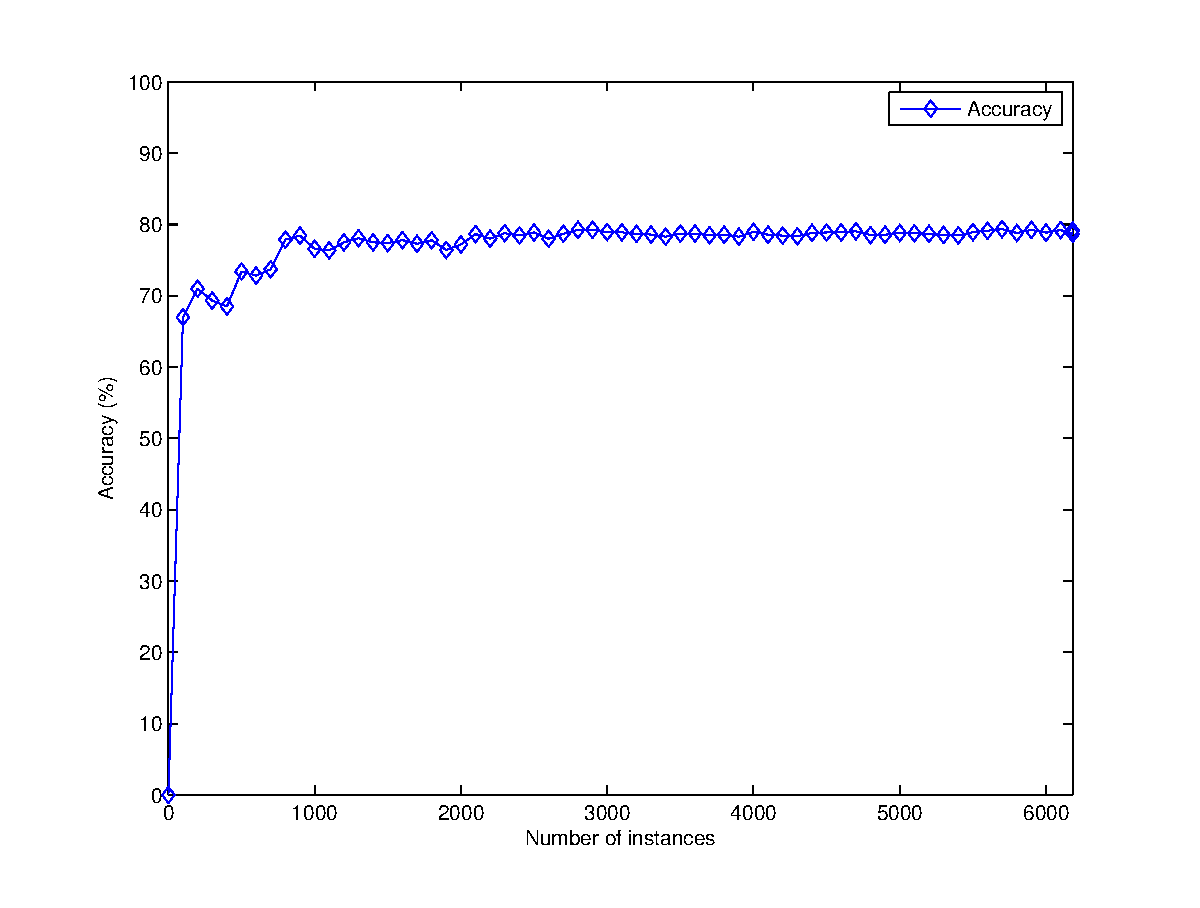
\includegraphics[scale=0.5]{svm_accuracy.eps}
    \caption{Accuracy of a linear kernel measured against the number of instances} \label{svm_accuracy}
\end{figure}

Plot number of instances against -
\begin{itemize}
    \item{accuracy}
    \item{number of suppor vectors}
\end{itemize}
depending on which kernel is being used.

\subsection{Ensemble Learning}
Ensemble learning methods are evaluated.

Plot number of instances against -
\begin{itemize}
    \item{accuracy}
\end{itemize}

Plot accuracy against -
\begin{itemize}
    \item{number of models in the ensemble}
    \item{sample weights (MATLAB plots from Han's implementation)}
\end{itemize}

\subsubsection{Bagging}
results from bagging

\subsubsection{Boosting}
results from boosting

\subsubsection{Stacking}
results from stacking

\section{System Details}

The second major contribution of this thesis is a web based system that allows users to perform (broadly) the following functions - help build the training data, evaluate a level of distress amongst the general public, and find out particular people who have been posting content that appears to be distressed and qualifies as needing-attention.

Specifically, users can assign labels to stories fetched from reddit, which helps in building training data while tapping into crowd intelligence. The \emph{monitoring} module then presents information about a general level of distress amongst people who are posting on Twitter (grouped by date), and about certain tweets that have been classified as depressed. Showing information about particular tweets which have been classified as depressed presents authors of the tweet which may need further attention in the form of psychological help.

The system is divided into two modules - \emph{Ratings} and \emph{Monitoring}. This choice is presented to a user as soon as they visit the front page of the web interface, as shown in Figure~\ref{landing}.
\begin{figure}
    \centering
        \includegraphics[width=\textwidth,scale=0.5]{landing.png}
    \caption{Landing page} \label{landing}
\end{figure}

The flow of the entire system can be seen as being divided into two parts. The first part, which is more manual, includes users fetching stories (from reddit) and labelling them, which helps in building the training data. The second part is built using automatic cron jobs (pieces of code that are executed after specific intervals of time), and involves the following -
\begin{itemize}
    \item{every 3 hours - fetching 100 tweets from the public stream of Twitter}
    \item{every morning - assigning labels to all tweets fetched from Twitter according to the updated model}
\end{itemize}

\section{Ratings}
The \emph{Ratings} module is built to help consolidate the training data. Users are provided with options to label the unlabeled data (as ``depressed'' or ``not depressed'') that is already present in the database. If in case there are no unlabeled stories left, then there also exists an option to fetch more data from Reddit. When invoked, this option fetches 500 stories each from \href{http://www.reddit.com/r/happy}{/r/happy} and \href{http://www.reddit.com/r/suicidewatch}{/r/suicidewatch}.

As shown in Figure~\ref{ratings}, the user is presented with a random piece of text that was fetched from Reddit, and two buttons for assigning this story a label.

\begin{figure}
    \centering
        \includegraphics[width=\textwidth,scale=0.5]{ratings.png}
    \caption{Ratings module} \label{ratings}
\end{figure}

\section{Monitoring}
